The location proof system I propose allows \textit{mobile nodes} to create location proofs by initiating an \textit{exchange} with another anonymous mobile node. When two mobile nodes are in close physical proximity, they initiate an exchange in the background over a short range, ad-hoc network such as Bluetooth. On completion of the exchange, both nodes can generate their own \textit{transaction}, a cryptographically secure proof of location, attested by the other mobile node.

To create a transaction, two mobile nodes anonymously exchange their GPS coordinates and current time over the ad-hoc network. Both nodes then check that these parameters don't differ from their own observed parameters by more than some value $\epsilon$. Once satisfied, they each create an encrypted, privacy-protecting transaction logging their location and the identity of the other mobile node (the \textit{alibi}) used to create the transaction. This transaction is published onto a public, append-only bulletin board known as a \textit{blockchain} \cite{blueprint}. Once given permission from a mobile node, a \textit{Verifier node} can consult the data in blockchain and determine whether or not the mobile node is present at its claimed location.

Any mobile node acting as an alibi in a transaction will share details of its most recent transactions with the other mobile node in the exchange. This means that when the mobile node seeks verification from a Verifier node, the Verifier can examine the mobile node's alibi's, and each of the alibi's recent alibi's, forming a large tree of connections which can be used to verify or reject the mobile nodes claimed location. Only the owner of the transaction can give permission to a Verifier to check its location history, by providing the Verifier with the keys needed to decrypt the transactions.

Figure \ref{fig:overview} provides an overview of the operation of the proposed system.

\begin{figure}[H]
\begin{center}
\resizebox {\columnwidth} {!} {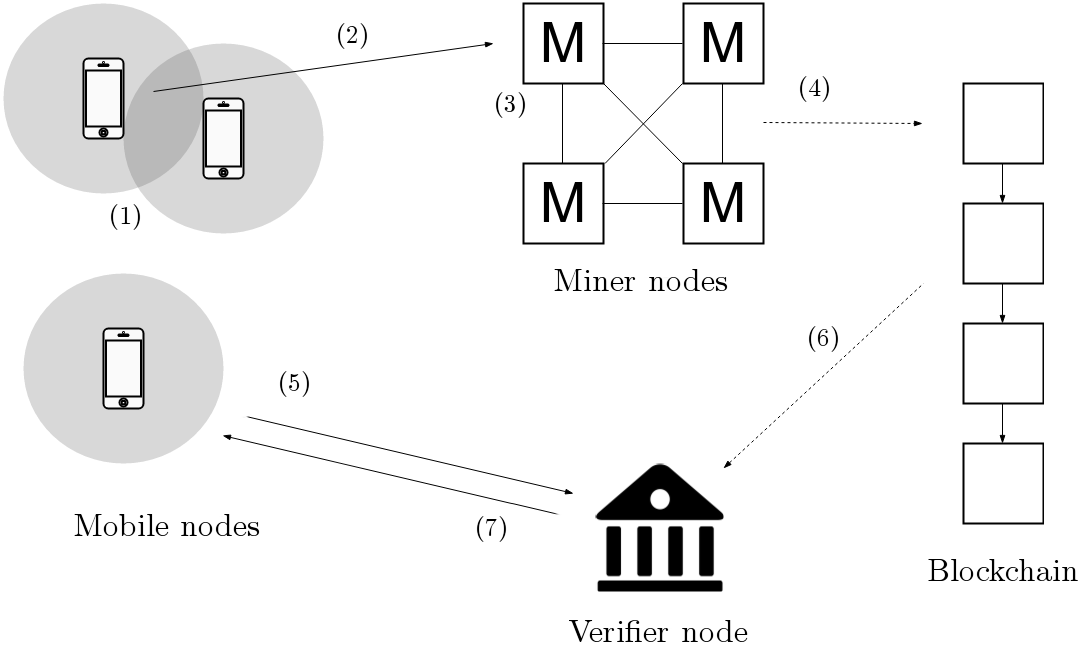
\includegraphics{diagrams/overview.png}}
\caption{Design and operation overview}
\label{fig:overview}
\end{center}
\end{figure}

\begin{enumerate}[label=\textbf{\arabic*}.]
\item Two mobile nodes come in close physical proximity and create an ad-hoc network, over which they initiate an exchange and each create a transaction.
\item Both mobile nodes publish their own transaction to a Miner node.
\item The Miner node who received the transaction distributes it across the Miner network.
\item One Miner node solves the proof-of-work for a block of transactions, and the new block is appended to the blockchain.
\item A mobile node requests verification from a Verifier node (request structure is explained in section \ref{ssec:verification}).
\item The Verifier node uses the public blockchain to examine the requesting node's transactions and determine their validity.
\item The Verifier accepts or rejects the  mobile node's claimed location based on its analysis of the transactions in the blockchain. 
\end{enumerate}

\section{Identities}
In order to preserve user's privacy, a user will only ever use an identity for one transaction, before generating a new one. This prevents curious users from watching the public blockchain for a known identity and tracking it. However, to prevent identity theft, it is important for the Verifier to be able to prove that a mobile node is the owner of each identity. This is achieved using a public/private key pair for each mobile node.

When a mobile node is first joins the network, it generates a public/private key pair. To maintain anonymity, the mobile node will use the public key to encrypt \textit{nonces} to create \textit{identities}, and use these to identify itself in a transaction. A different identity will be created for each transaction. During the verification stage, the node will provide the Verifier with its public key, along with the list of the nonces used to generate its $n$ most recent transactions (see figure \ref{fig:verify_request}). This allows the Verifier to calculate all of the node's identities, and prove that they were all created by the same node. The Verifier can then retrieve the transactions associated with those identities from the blockchain. The Verifier will also ensure that the node owns the private key associated with the provided public key, to prevent a weak identity attack.

\subsection{Nonce list} \label{sssec:nonce_list}
A \textit{Nonce List} is simply a list of all of the nonces a mobile node has used so far to generate identities. When a mobile node wishes to generate a new identity, it must first generate a new nonce which is then encrypted to create the identity. The nonce is appended to the mobile node's nonce list, so it can be used later during verification (see section \ref{ssec:verification}).

\begin{figure}[H]
\resizebox {\columnwidth} {!} {\documentclass[border=2pt]{standalone}
\usepackage{tikz}
\usetikzlibrary{matrix,positioning,arrows.meta,arrows,calc}

\tikzset{
mymat/.style={
  matrix of math nodes,
  text height=2.5ex,
  text depth=0.75ex,
  text width=5.25ex,
  align=center,
  column sep=-\pgflinewidth
  },
mymats/.style={
  mymat,
  text width=8ex,
  nodes={draw}
  }  
}
\begin{document}

\begin{tikzpicture}[>=latex]
\matrix[mymat,anchor=west,row 1/.style={nodes=draw}]
at (0,0) 
(mat1)
{
4827 & 1928 & 9183 & 0047\\
};
\matrix[mymats=white,anchor=west]
at (0,-3) 
(mat3)
{
12ef5a1 & c100e9d & 038ef6b & ee3bc14 \\
};

\node[left=0pt of mat1]
  (cella) {Nonce list:};
  
\node[left=0pt of mat3]
  (cella) {Identities:};
  
  
\node (key) at ($(mat1-1-4.south)!0.5!(mat3-1-4.north)$) {$K^+(0047)$};

\begin{scope}[shorten <= -2pt]
\draw[*->]
  (mat1-1-1.south) -- (mat3-1-1.north);
\draw[*->]
  (mat1-1-2.south) -- (mat3-1-2.north);
\draw[*->]
  (mat1-1-3.south) -- (mat3-1-3.north);
\draw[*-]
  (mat1-1-4.south) -- (key);
\draw[->]
  (key) -- (mat3-1-4.north);
\end{scope}
\end{tikzpicture}

\end{document}}
\caption{Identity generation from Nonce List}
\label{fig:nonce_list}
\end{figure}

In figure \ref{fig:nonce_list} above, nonce $0047$ is encrypted with $K^+$ to create identity $ee3bc14$. By providing the nonce list and $K^+$, a node can prove that it created all of the identities in the identities list. It must also verify that it owns $K^-$, its private key.

\subsection{Identity duplication}
Since all identities are generated from random nonces, there is nothing to prevent two nodes from generating the same identity and using it in different transactions. It is therefore possible that during verification, a Verifier node may find multiple transactions with the same ID while searching the blockchain. The Verifier will have a decryption key for the transaction it is searching for, which will only successfully decrypt one of the transactions with the duplicate ID. The Verifier will try to decrypt each one until it finds the one that can be decrypted successfully.

\newpage
\section{Transactions} \label{sec:transactions}
During an exchange between two nodes, a number of different items must be shared and calculated. Figure \ref{fig:transaction} describes and explains an honest, successful exchange, assuming an ad-hoc Bluetooth network has already been set up between nodes $A$ and $B$.

\begin{figure}[H]
\begin{center}
\resizebox {1.1\columnwidth} {!} {\begin{tikzpicture}
\coordinate (A_1) at (0,10);
\coordinate (A_2) at (0,9.5);
\coordinate (A_3) at (0,9);
\coordinate (A_4) at (0,8.5);
\coordinate (A_5) at (0,8);
\coordinate (A_6) at (0,7.5);
\coordinate (A_7) at (0,7);
\coordinate (A_8) at (0,4.5);
\coordinate (A_9) at (0,4);
\coordinate (A_10) at (0,1.5);
\coordinate (A_11) at (0,0.25);
\coordinate (A_12) at (0,0);
\coordinate (AF_L) at (-0.25,0);
\coordinate (AF_R) at (0.25,0);

\coordinate (M_1) at (3.5,8.5);
\coordinate (M_2) at (3.5,7.5);

\coordinate (B_1) at (7,10);
\coordinate (B_2) at (7,9.5);
\coordinate (B_3) at (7,9);
\coordinate (B_4) at (7,8.5);
\coordinate (B_5) at (7,8);
\coordinate (B_6) at (7,7.5);
\coordinate (B_7) at (7,7);
\coordinate (B_8) at (7,6);
\coordinate (B_9) at (7,5.5);
\coordinate (B_10) at (7,1.5);
\coordinate (B_11) at (7,0.25);
\coordinate (B_12) at (7,0);
\coordinate (BF_L) at (6.75,0);
\coordinate (BF_R) at (7.25,0);

\draw[thick] (A_1)--(A_2) (A_3)--(A_4) (A_5)--(A_6) (A_7)--(A_8) (A_9)--(A_10) (A_11)--(A_12) (AF_L)--(AF_R);
\draw[thick] (B_1)--(B_2) (B_3)--(B_4) (B_5)--(B_6) (B_7)--(B_8) (B_9)--(B_10) (B_11)--(B_12) (BF_L)--(BF_R);
\draw (A_1) node[above]{\Large Node $A$};
\draw (B_1) node[above]{\Large Node $B$};

\draw ($(A_1)!.5!(A_2)$) node[left]{\begin{tabular}{r}
\textit{$KL_{A1}$, $KL_{A2}$}
\end{tabular}};

\draw ($(B_1)!.5!(B_2)$) node[right]{\begin{tabular}{r}
\textit{$KL_{B1}$, $KL_{B2}$}
\end{tabular}};

\draw (A_2) node[below,text centered]{\begin{tabular}{r}
\small{\textit{generate $ID_{An}$}}
\end{tabular}};

\draw (B_2) node[below,text centered]{\begin{tabular}{r}
\small{\textit{generate $ID_{Bm}$}}
\end{tabular}};

\draw (M_1) node[below,text centered]{\begin{tabular}{r}
bluetooth advertising and scanning
\end{tabular}};

\draw (M_2) node[below,text centered]{\begin{tabular}{r}
ad-hoc network established between $A$ and $B$
\end{tabular}};

\coordinate (AX_1) at ($(A_7)-(0,0.25)$);
\coordinate (BX_1) at ($(B_7)-(0,0.5)$);
\draw[->] (AX_1) -- (BX_1) node[midway,below]
	{$T_{req}$: $ID_{An} | ts_A | loc_A$};
	
\draw (B_8) node[below,text centered]{\begin{tabular}{r}
\small{\textit{verify $|ts_A-ts_B| < \epsilon_{ts}$ and $|loc_A-loc_B| < \epsilon_{loc}$}}
\end{tabular}};

\coordinate (AX_2) at ($(A_7)-(0,2)$);
\coordinate (BX_2) at ($(B_9)-(0,0.25)$);
\draw[->] (BX_2) -- (AX_2) node[midway,below]
	{$T_{res}$: $ID_{Bn} | ts_A | loc_A$};
	
\draw (A_8) node[below,text centered]{\begin{tabular}{r}
\small{\textit{verify $|ts_A-ts_B| < \epsilon_{ts}$ and $|loc_A-loc_B| < \epsilon_{loc}$}}
\end{tabular}};

\coordinate (AX_3) at ($(A_9)-(0,0.25)$);
\coordinate (BX_3) at ($(B_9)-(0,2)$);
\draw[->] (AX_3) -- (BX_3) node[midway,below]
	{$ID_{An-1}|KP_{An}$};

\coordinate (AX_4) at ($(A_9)-(0,1.5)$);
\coordinate (BX_4) at ($(B_9)-(0,2.75)$);
\draw[->] (BX_4) -- (AX_4) node[midway,below]
	{$ID_{Bm-1}|KP_{Bm}$};

\draw (A_10) node[below,text centered]{\begin{tabular}{r}
\small{\textit{$T_{An}$ = $KL_{A2}[n](ts|loc|ID_{An}|KP_{Bm})$}}\\
\small{\textit{publish $ID_{An}|KL_{A1}[n](ID_{An-1})|T_{An}$}}
\end{tabular}};

\draw (B_10) node[below,text centered]{\begin{tabular}{r}
\small{\textit{$T_{Bm}$ = $KL_{B2}[m](ts|loc|ID_{Bm}|KP_{An})$}}\\
\small{\textit{publish $ID_{Bm}|KL_{B1}[m](ID_{Bm-1})|T_{Bm}$}}
\end{tabular}};
\end{tikzpicture}}
\caption{Honest, successful exchange}
\label{fig:transaction}
\end{center}
\end{figure}

\begin{itemize}
	\item[] \textbf{(1)} Before the exchange begins, both nodes generate a new entry in their nonce list (e.g. $NL_A[n]$), and generate a new identity from that nonce (e.g. $ID_A[n]$).
	\item[] \textbf{(2)} Node A sends its identity to Node B, along with its observed current timestamp $ts_A$ and current GPS location $loc_A$.
	\item[] \textbf{(3)} Node B verifies that the observed timestamp and GPS location received from Node A are within an acceptable difference from its own observations. This difference is defined by some system constant $\epsilon$.
	\item[] \textbf{(4)} If Node B verifies the parameters received from Node A, it will respond with its own identity and observations for A to verify.
	\item[] \textbf{(5)} Node A verifies that the parameters received from B differ by no more than $\epsilon$ from its own observed parameters.
	\item[] \textbf{(6)} Node A sends $KP_{An}$, its $nth$ \textit{Key Packet}. Key Packets are used to provide alibi credibility, and are discussed in section \ref{sssec:key_packets}.
	\item[] \textbf{(7)} B responds with its own Key Packet.
	\item[] \textbf{(8)} Both nodes generate their own transaction $T$, using their alibi's Key Packets. These are then used to generate $P$, the data published onto the public blockchain.
\end{itemize}

\subsection{Key Lists} \label{ssec:key_lists}
When a node is initialised, it must begin to record two \textit{Key Lists} for itself. A \textit{Key List} is a list of encryption keys previously used for transactions. For example, $KL_{AT}[n]$ and $KL_{AL}[n]$ are the two keys used to encrypt node $A$'s $n$th transaction and matching chronological link, respectively. These \textit{Key Lists} and are assumed to have been initialised and populated before the transaction described in Figure \ref{fig:transaction} begins.

\subsection{Transaction creation}
Once nodes have exchanged \textit{Key Packets}, their communication is finished and they can close their ad-hoc channel. Each node creates a new transaction, $T$, and generates data $P$ to publish onto the public blockchain. The following transaction will be created by node $A$, after communicating with node $B$:
\\

$T_{An} = KL_{AT}[n](ts|loc|ID_{A}[n]|ID_{B}[m]|KP_{Bm})$
\\

Where:
\begin{itemize}[noitemsep,topsep=0pt]
	\item[] $\mathbf{n}$ is node $A$'s current transaction number (i.e. $A$ has published $n-1$ transactions before now).
	\item[] $\mathbf{KL_{AT}}$ is $A$'s transaction \textit{Key Lists}, used to encrypt transactions.	
	\item[] $\mathbf{ts}$ is the timestamp of the transaction, as recorded by node $A$.
	\item[] $\mathbf{loc}$ is the GPS coordinates of the transaction, as recorded by node $A$.
	\item[] $\mathbf{ID_{A}[n]}$ is $A$'s $nth$ identity, used for this transaction only.
	\item[] $\mathbf{ID_{B}[m]}$ is $B$'s $mth$ identity.
	\item[] $\mathbf{KP_{Bm}}$ is $B$'s \textit{Key Packet} at time $m$. Its exact contents are discussed in more detail in section \ref{sssec:key_packets}
\end{itemize}

\subsection{Publishing to the blockchain}
After creating $T_{An}$, node $A$ must publish it to the public blockchain. The data published must be searchable in order to provide a Verifier with some way of identifying specific transactions. Nodes use their current ID as the identifier for the transaction.

\textit{Backwards-chaining} is an important part of verifiability. The Verifier must be able to prove that the proof chain provided by the mobile node has not been chronologically re-ordered. This is the ``order preserving'' property of OTIT \cite{otit}. The transaction must therefore be accompanied by a link to the node's chronologically previous transaction. This link is encrypted with $KL_{AL}[n]$, $A$'s $nth$ \textit{link} key list, to prevent a curious user from monitoring the public blockchain to observe a user's transaction publishing activity. The timestamp $ts_A$ is also included in the backwards-chaining data, to verify the ``order preserving'' property. $A$'s transaction data $P_{An}$ will therefore be in the form:
\\

$P_{An} = ID_{An}|KL_{AL}[n](ID_{A}[n-1]|ts_A)|T_{An}$

\null
To publish $P_{An}$, $A$ must send $P_{An}$ to a miner node, who will add it to its \textit{pending transaction} queue, and send it to other miners in the network to add it to their queues as well. The transaction will signed into the next block in the blockchain, once the next proof-of-work is solved.

Node $B$, $A$'s alibi for the above transaction example, will publish $P_{Bm}$ after the exchange. If $B$'s transaction is not available on the blockchain, $A$'s transaction will be considered invalid and disregarded during verification. A transaction $T_A$ in the blockchain must be accompanied by a reference to some valid alibi transaction $T_B$, and $T_B$ must reference $T_A$, otherwise the proof is not considered credible by a verifier.

\subsection{Key Packets} \label{sssec:key_packets}
The key packet is more than simply a list of keys that a mobile node has used to encrypt its transactions; in order to preserve the ``selective in-sequence privacy'' property of OTIT \cite{otit}, a user must be able to choose transactions that he doesn't want others to be able to decrypt. However, in order to simultaneously preserve OTIT's ``privacy protected chronology'' property, the transaction backwards-chaining must not be broken. This is why two separate \textit{Key Lists} are maintained; $KL_{AL}$ is used to encrypt the backwards-chaining link and transaction timestamp, while $KL_{AT}$ encrypts the transaction data. For example, if node $B$ doesn't want to reveal transaction $T_{Bm-1}$, he would reveal the following key packet:
\\

${KP_{Bm} = (\{KL_{BL}[m], KL_{BT}[m]\}, KL_{BL}[m-1], \{KL_{BL}[m-2], KL_{BT}[m-2]\})}$

\null
In this case, $KL_{BT}[m-1]$ has not been included with $KL_{BL}[m-1]$, in order to protect the privacy of this transaction. This means that a node who received this key packet will not be able to decrypt $B$'s transaction $T_{Bm-1}$, but can still prove that a transaction exists at that time and in the correct sequence, as $B$ will still provide $KL_{BL}[m-1]$. This may be needed, for example, if node $B$ doesn't want to allow anyone to decrypt any transactions he has created within 5km of his home, in order to protect his privacy.

\subsection{Aborting exchanges} \label{ssec:aborting_exchanges}
A node may decide to abort an exchange if it thinks it is in contact with a malicious node. In figure \ref{fig:aborted_transaction}, node $A$ encounters a malicious node $M$, who tries to spoof its identity with $A$. Node $A$ will abort the exchange once it notices that $|ts_A-ts_M| \geq \epsilon_{ts}$, or $|loc_A-loc_M| \geq \epsilon_{loc}$.

To abort the exchange, $A$ terminates the ad-hoc network with node $M$, and won't publish anything onto the blockchain. This means that even if $M$ fabricates some data from $A$ and publishes a transaction onto the blockchain, the matching transaction from $A$ will not be present, so $M$'s transaction will be disregarded by any verifiers.

\begin{figure}
\resizebox {\columnwidth} {!} {\begin{tikzpicture}
\coordinate (A_1) at (0,5.5);
\coordinate (A_2) at (0,5.25);
\coordinate (A_3) at (0,4.5);
\coordinate (A_8) at (0,1);
\coordinate (A_9) at (0,0.25);
\coordinate (A_12) at (0,0);
\coordinate (AF_L) at (-0.25,0);
\coordinate (AF_R) at (0.25,0);

\coordinate (B_1) at (8,5.5);
\coordinate (B_3) at (8,4.5);
\coordinate (B_8) at (8,3.25);
\coordinate (B_9) at (8,2.5);
\coordinate (B_12) at (8,0);

\draw[thick] (A_1)--(A_2) (A_3)--(A_8) (A_9)--(A_12) (AF_L)--(AF_R);
\draw[thick] (B_1)--(B_3) (B_3)--(B_9) (B_9)--(B_12);
\draw (A_1) node[above]{\Large Node $A$};
\draw (B_1) node[above]{\Large Malicious node $M$};

\draw (A_2) node[below,text centered]{\begin{tabular}{r}
\small{\textit{generate $NL_A[n]$, $ID_{An} = K^{+}_A(NL_A[n])$}}
\end{tabular}};

\coordinate (AX_1) at ($(A_3)-(0,0.5)$);
\coordinate (BX_1) at ($(B_3)-(0,1)$);
\draw[->] (AX_1) -- (BX_1) node[midway,below]
	{$T_{req}$: $ID_{An} | ts_A | loc_A$};

\coordinate (AX_2) at ($(A_3)-(0,3)$);
\coordinate (BX_2) at ($(B_8)-(0,1)$);
\draw[->] (BX_2) -- (AX_2) node[midway,below]
	{$T_{res}$: $ID_{M} | ts_M | loc_M$};
	
\draw (A_8) node[below,text centered]{\begin{tabular}{r}
\small{\textit{verify $|ts_A-ts_M| < \epsilon_{ts}$, $|loc_A-loc_M| < \epsilon_{loc}$}}
\end{tabular}};
\end{tikzpicture}}
\caption{An aborted transaction due to malicious node $M$}
\label{fig:aborted_transaction}
\end{figure}

\clearpage
\section{Verification} \label{ssec:verification}
In the verification stage, a mobile node tries to prove its location to a Verifier node, e.g. a bank. To do this, the mobile node sends the Verifier a number of parameters, as shown in Figure \ref{fig:verify_request}.

\begin{figure}[H]
\begin{center}
\resizebox {0.8\columnwidth} {!} {\begin{tikzpicture}
\coordinate (A_1) at (0,6);
\coordinate (A_2) at (0,0);

\coordinate (B_1) at (6,6);
\coordinate (B_2) at (6,1.75);
\coordinate (B_3) at (6,1);
\coordinate (B_4) at (6,0);

\draw[thick] (A_1)--(A_2);
\draw[thick] (B_1)--(B_2) (B_3)--(B_4);
\draw (A_1) node[above]{\Large Node $A$};
\draw (B_1) node[above]{\Large Verifier};

\coordinate (AX_1) at ($(A_1)-(0,0.5)$);
\coordinate (BX_1) at ($(B_1)-(0,0.75)$);
\draw[->] (AX_1) -- (BX_1) node[midway,below]
	{$ID_{An-1}|KP_{An-1}|loc|NP_{An-1}|K^{+}_A$};
	
\coordinate (AX_2) at ($(A_1)-(0,2.25)$);
\coordinate (BX_2) at ($(B_1)-(0,2)$);
\draw[->] (BX_2) -- (AX_2) node[midway,below]
	{$K^{+}_A(nonce)$};

\coordinate (AX_3) at ($(A_1)-(0,3.25)$);
\coordinate (BX_3) at ($(B_1)-(0,3.5)$);
\draw[->] (AX_3) -- (BX_3) node[midway,below]
	{$K^{-}_A(K^{+}_A(nonce))$};
	
\draw (B_2) node[below,text centered]{\begin{tabular}{r}
consult blockchain
\end{tabular}};

\coordinate (AX_2) at ($(A_1)-(0,5.5)$);
\coordinate (BX_2) at ($(B_1)-(0,5.25)$);
\draw[->] (BX_2) -- (AX_2) node[midway,below]
	{verify or reject};

\end{tikzpicture}}
\caption{Verification request}
\label{fig:verify_request}
\end{center}
\end{figure}

\begin{itemize}[noitemsep,topsep=0pt]
	\item[] $\mathbf{ID_{A}[n-1]}$ is the ID of $A$'s most recently published transaction.
	\item[] $\mathbf{KP_{An-1}}$ is $A$'s key packet up to transaction $n-1$, and includes keys for as many transactions as $A$ feels is appropriate in order to receive verification.
	\item[] $\mathbf{loc}$ is $A$'s current claimed GPS coordinates for which it is seeking verification.
	\item[] $\mathbf{NP_{An-1}}$ is $A$'s \textit{Nonce Packet}, a subset of its \textit{Nonce List} (section \ref{sssec:nonce_list}). A Nonce Packet is the list of the nonces used to generate $A$'s most recent IDs, up to $n-1$, that $A$ is willing to share with the Verifier. 
\end{itemize}

\null
The goal of the verification stage is for the Verifier to either accept or reject the location that the user is claiming. Given $ID_{A}[n-1]$ and $KP_{An-1}$, a Verifier is able to retrieve $A$'s previous transactions, and the transactions of all of its alibi's. This will allow the Verifier to recursively inspect the transactions of all alibi's used in a nodes transactions, until it is satisfied that the location can be verified or rejected. This recursive inspection can be visualised as a tree, as shown in figure \ref{fig:tree}.

\begin{figure}[H]
\begin{center}
\resizebox {0.7\columnwidth} {!} {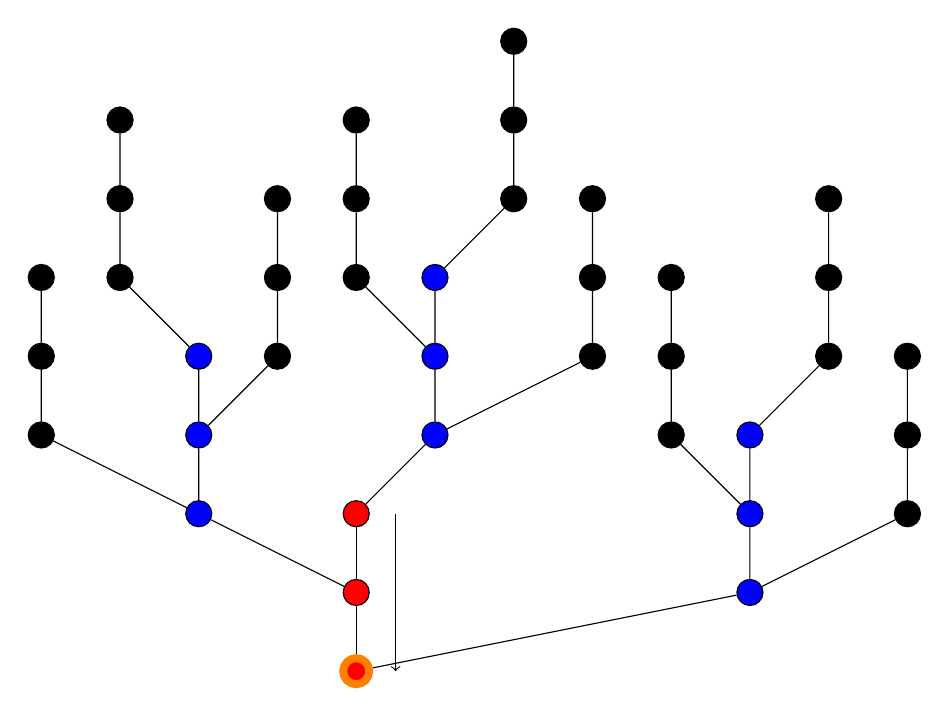
\begin{tikzpicture}[every node/.style={draw,shape=circle,fill=black}]

\node[fill=red,line width=1mm,draw=orange] (A) at (0,0) {};
\node[fill=red] (B) at (0,1) {};
\node[fill=red] (C) at (0,2) {};

\draw (A) -- (B) (B) -- (C);

\only<2> {
\draw[->] (0.5,2) -- (0.5,0);
}

\onslide<3->{
\node[fill=blue] (D) at (5,1) {};
\node[fill=blue] (E) at (5,2) {};
\node[fill=blue] (F) at (5,3) {};

\draw (A) -- (D) (D) -- (E) (E) -- (F);

\node[fill=blue] (G) at (-2,2) {};
\node[fill=blue] (H) at (-2,3) {};
\node[fill=blue] (I) at (-2,4) {};

\draw (B) -- (G) (G) -- (H) (H) -- (I);

\node[fill=blue] (J) at (1,3) {};
\node[fill=blue] (K) at (1,4) {};
\node[fill=blue] (L) at (1,5) {};

\draw (C) -- (J) (J) -- (K) (K) -- (L);
}

\onslide<4->{
\node (M) at (-4,3) {};
\node (N) at (-4,4) {};
\node (O) at (-4,5) {};

\draw (G) -- (M) (M) -- (N) (N) -- (O);

\node (P) at (-1,4) {};
\node (Q) at (-1,5) {};
\node (R) at (-1,6) {};

\draw (H) -- (P) (P) -- (Q) (Q) -- (R);

\node (S) at (-3,5) {};
\node (T) at (-3,6) {};
\node (U) at (-3,7) {};

\draw (I) -- (S) (S) -- (T) (T) -- (U);

\node (V) at (0,5) {};
\node (W) at (0,6) {};
\node (X) at (0,7) {};

\draw (K) -- (V) (V) -- (W) (W) -- (X);

\node (Y) at (2,6) {};
\node (Z) at (2,7) {};
\node (AA) at (2,8) {};

\draw (L) -- (Y) (Y) -- (Z) (Z) -- (AA);

\node (AB) at (3,4) {};
\node (AC) at (3,5) {};
\node (AD) at (3,6) {};

\draw (J) -- (AB) (AB) -- (AC) (AC) -- (AD);

\node (AE) at (4,3) {};
\node (AF) at (4,4) {};
\node (AG) at (4,5) {};

\draw (E) -- (AE) (AE) -- (AF) (AF) -- (AG);

\node (AH) at (6,4) {};
\node (AI) at (6,5) {};
\node (AJ) at (6,6) {};

\draw (F) -- (AH) (AH) -- (AI) (AI) -- (AJ);

\node (AK) at (7,2) {};
\node (AL) at (7,3) {};
\node (AM) at (7,4) {};

\draw (D) -- (AK) (AK) -- (AL) (AL) -- (AM);
}

\end{tikzpicture}}
\vspace{-3cm}
\caption{Alibi chain relationship tree}
\label{fig:tree}
\end{center}
\end{figure}

If the verifier wishes to recurse more, it could inspect the black node's alibis' transaction chains. Note that this is a simple example, and $n = 3$, the length of the transaction chain subset provided for verification. In reality $n$ should be much larger.

The Verifier uses $NP_{An-1}$ and $K^{+}_A$ to prove that node $A$ was the author of all of the transactions he claims to be. This prevents a collusion attack whereby nodes could share common transactions between different proof chains. When walking chronologically backwards along $A$'s proof chain, the 3rd party will ensure that the ID used in transaction $m$ on the proof chain matches $K^{+}_A(NP_{An-1}[m])$.

There are a huge number of possible factors involved in reaching a conclusion from the data on the blockchain; some of these factors will likely be unique to certain Verifiers, and kept secret to improve reliability and avoid gaming. Some simple example factors may include:
\begin{itemize}
	\item \textbf{Alibi credibility:} if each of the node’s alibi’s have little or no alibi’s themselves, they won't be considered credible alibis, and the Verifier will reject his verification request.
	\item \textbf{Transaction relevance:} if the Verifier considers the transactions it receives to be out of date, they will be rejected on the grounds that they are no longer relevant.
	\item \textbf{Alibi reuse:} if the Verifier can prove that alibi’s are being reused frequently, then it will reject the verification request.
	\begin{itemize}
		\item Due to transaction anonymity, the Verifier may not always be able to tell if two alibi's are the same person or not. e.g. node $A$ could use node $B$ as an alibi, then wait for $B$ to complete $n$ more transactions, then use node $B$ again.
		\item This is not a viable attack on the verification system. Depending on the size of $n$, enough time may pass between both uses of node $B$ as an alibi that the transactions are no longer relevant.
	\end{itemize}
\end{itemize}